\section{Sensor de corriente}

    Para poder usar el convertidor reductor explicado en la sección
    \ref{sec:buck_design} es necesario medir la corriente que se
    está entregando a la batería. Para ello se diseñó un sensor de corriente
    basado en el amplificador operacional TL082.

    El sensor tiene 3 componentes principales, el amplificador diferencial, 
    la resistencia de sensado y un filtro RC para eliminar el ruido de conmutación
    en la resistencia de sensado. El amplificador diferencial se encarga de 
    amplificar la diferencia de potencial entre los terminales de la resistencia
    de sensado, la cual es proporcional a la corriente que circula por la misma.
    La resistencia de sensado tiene un valor de $15 \text{m}\Omega$, con una
     tolerancia de $\pm 5\%$. Para el filtro RC se escogió una frecuencia de corte
     de $7.96\text{kHz}$, con el cual es posible eliminar el ruido de conmutación
    en la resistencia de sensado, la frecuencia de corte escogida
    se debe a 2 razones, la primera es que la frecuencia de conmutación del
    convertidor reductor es de $150\text{kHz}$, y la segunda es que no se desea
    que las resistencias del filtro RC sean de valor alto con relación a las
    resistencias del amplificador diferencial, ya que esto puede afectar la
    precisión del sensor, por lo que se escogió que las resistencias del filtro
    RC sean de $10\Omega$.

    Para poder medir una corriente máxima de $1.5\text{A}$ se escogió que 
    la ganancia para el amplificador diferencial (ver figura \ref{fig:ampDif})
    sea de $200\text{V/V}$, por lo que la salida del sensor será de
    $4.5\text{V}$ cuando la corriente sea de $1.5\text{A}$. Para obtener
    la ganancia deseada, se calcularon los valores de resistencia 
    necesarios utilizando la Ecuación \ref{eq:ampDifSimp}, fijando 
    el valor de $R_2$ en
    $1.5\text{K}\Omega$, obteniendo que el valor de $R_4$ debe ser de 
    $300\text{K}\Omega$. Debido a la  simplificación del circuito hecha en la 
    sección \ref{sec:ampDif} el valor de $R_1$ debe ser de $1.5\text{K}\Omega$
    y el valor de $R_3$ debe ser de $300\text{K}\Omega$. El sensor de corriente 
    diseñado se muestra en la figura \ref{fig:sensor_corriente}.

    \begin{figure}[H]
        \centering
        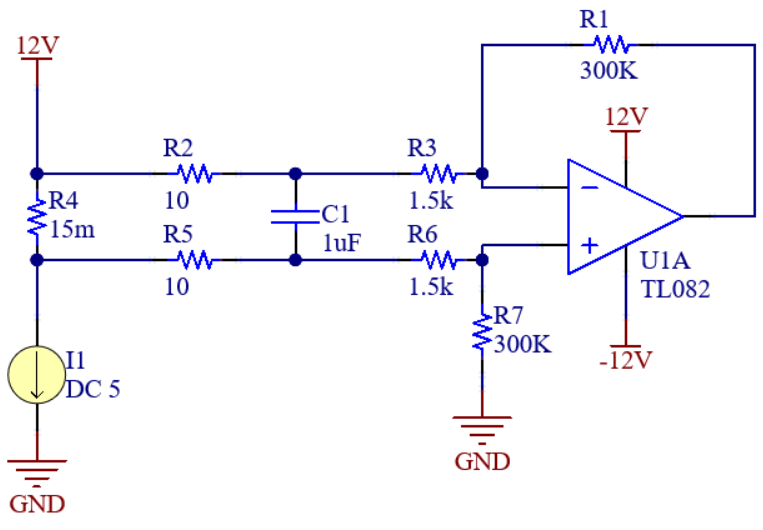
\includegraphics[scale=0.5]{imagenes/current_sensor.png}
        \caption{Sensor de corriente diseñado}
        \label{fig:sensor_corriente}
    \end{figure}

    con lo explicado anteriormente, el sensor tiene una ganancia final de 
    $3\text{V/A}$, la ecuación \ref{eq:sensor} describe la relación entre
    la corriente que circula por la resistencia de sensado y el voltaje de salida
    del amplificador diferencial.

    \begin{equation}
        V_{out} = 3I_1
        \label{eq:sensor}
    \end{equation}
    
    Para la alimentación del sensor es necesario un mínimo de $\pm7\text{V}$ en
    los pines de alimentación del amplificador operacional TL082, esto por dos 
    motivos, el primero es que el voltaje de salida del sensor es de $4.5\text{V}$
    cuando la corriente es de $1.5\text{A}$ tomando en cuenta que este opamp 
    no es del tipo \textit{rail to rail}, por lo que el voltaje de salida no
    puede ser igual al voltaje de alimentación, y el segundo motivo es que el
    voltaje en modo común de este amplificador tiene como limite superior el
    voltaje de alimentación positivo, por lo que es necesario que el voltaje 
    de alimentación sea mayor que el voltaje máximo de que recibirá en sus entradas,
    que para este caso es de $6.4\text{V}$. Para alimentar el sensor se empleó
    una alimentación simétrica de $\pm 12\text{V}$.
    
    \subsection{Mediciones del Sensor de corriente}

    Para comprobar el correcto funcionamiento del sensor de corriente diseñado
    se realizaron mediciones para varios niveles de corriente. Para ello se
    empleó una fuente de voltaje simétrica a $\pm7\text{V}$, y se utilizaron resistencias de entre 
    $4\Omega$ y $30\Omega$ para simular la carga de la batería. Los resultados 
    obtenidos son mostrados en la figura \ref{fig:mediciones_sensor_grap}. 

\begin{figure}[H]
    
    \centering     
    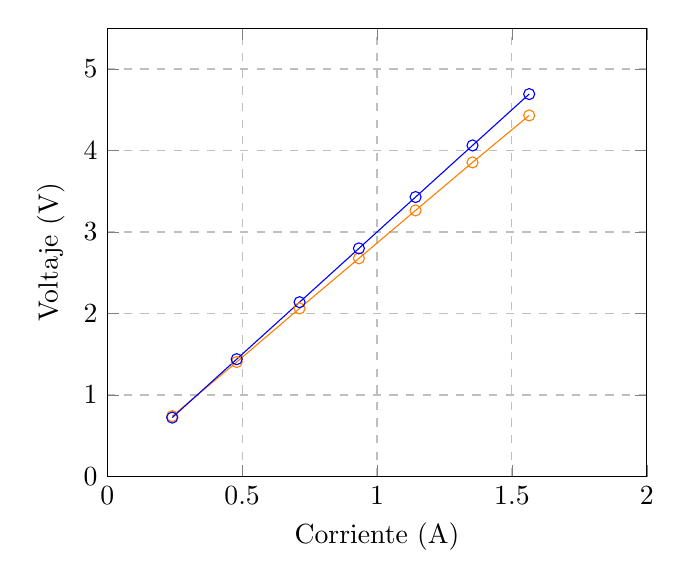
\begin{tikzpicture}
        
        \begin{axis}[
            xlabel={Corriente (A)},
            ylabel={Voltaje (V)},
            xmin=0, xmax=2,
            ymin=0, ymax=5.5,
            legend pos=north west,
            ymajorgrids=true,
            xmajorgrids=true,
            grid style=dashed,
        ]
     
    \addplot[color=orange,mark=o,]
        coordinates {
        (0.241,0.741)
        (0.480,1.405)
        (0.713,2.063)
        (0.933,2.677)
        (1.143,3.265)
        (1.354,3.854)
        (1.564,4.43)
        };
        \addplot[
            color=blue,
            mark=o,
            ]
            coordinates {
            (0.241,0.723)
            (0.480,1.440)
            (0.713,2.139)
            (0.933,2.799)
            (1.143,3.429)
            (1.354,4.062)
            (1.564,4.692)
            };
    \end{axis}
\end{tikzpicture}


\caption{Voltaje de salida del sensor de corriente (naranja valores medidos, azul valores esperados)}
\label{fig:mediciones_sensor_grap}
\end{figure}
 
En la figura \ref{fig:mediciones_sensor} se muestra el circuito construido
    en protoboard para la medición de los valores presentados anteriormente.

    \begin{figure}[H]
        \centering
        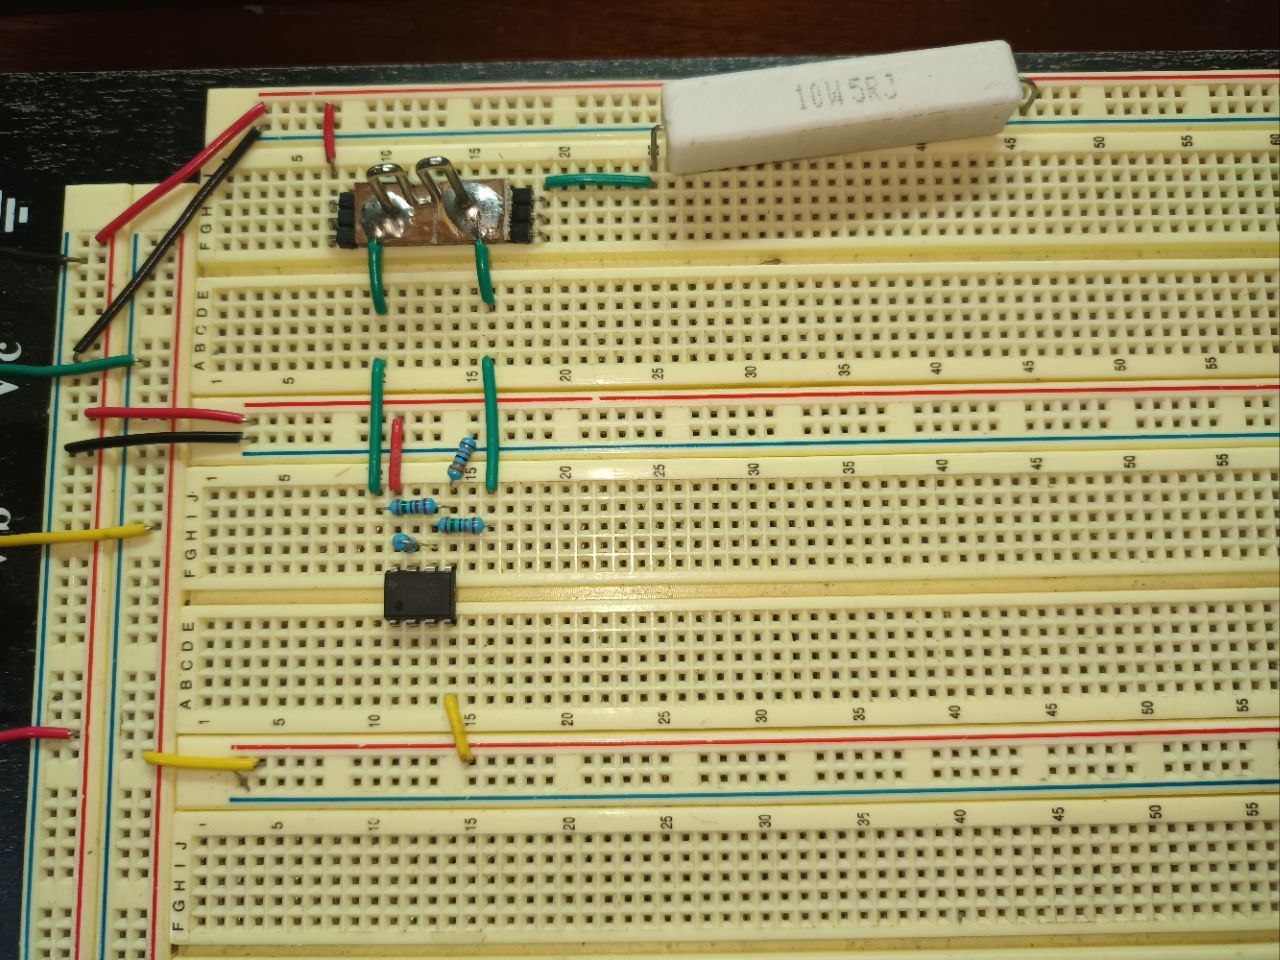
\includegraphics[scale=0.2]{imagenes/prueba_sensor.jpg}
        \caption{Circuito para medición del sensor de corriente}
        \label{fig:mediciones_sensor}
    \end{figure}
